\documentclass[10pt]{beamer}
\usetheme{jambro}

\title[]{Oferta e demanda agregada}
\author[]{Paulo Victor da Fonseca}
\date{06 de junho de 2023}

\hypersetup{
    colorlinks = true,
    urlcolor = teal,
    linkcolor = teal    
}
\usepackage[portuguese]{babel}
\usepackage{subfig}
\usepackage{emoji}
\usepackage{hyperref}

\begin{document}

\begin{frame}[plain]
    \titlepage{
        \begin{center}
            \begin{minipage}{0.8\textwidth}
                \centering
            \end{minipage}
        \end{center}}
\end{frame}

\begin{frame}{Sumário}
    \tableofcontents
\end{frame}

\section{Demanda agregada: curva IS}
\begin{frame}
    {Demanda agregada: curva IS}
    \begin{itemize}
        \item Curva IS: maneira sistemática de pensarmos como alterações no comportamento de gastos de firmas, consumidores e governos podem influenciar produto agregado e determinar ciclos econômicos\bigskip
        \item Mostra combinações de taxa de juros real e produto agregado para as quais o mercado de bens e serviços está em equilíbrio\bigskip
        \item Negativamente inclinada: decisões de consumo das famílias respondem negativamente a aumentos na taxa de juros; firmas incorrem em menos projetos de investimentos quando o custo de empréstimos aumenta
    \end{itemize}
\end{frame}

\begin{frame}
    {Demanda agregada: curva IS}
    \begin{figure}
        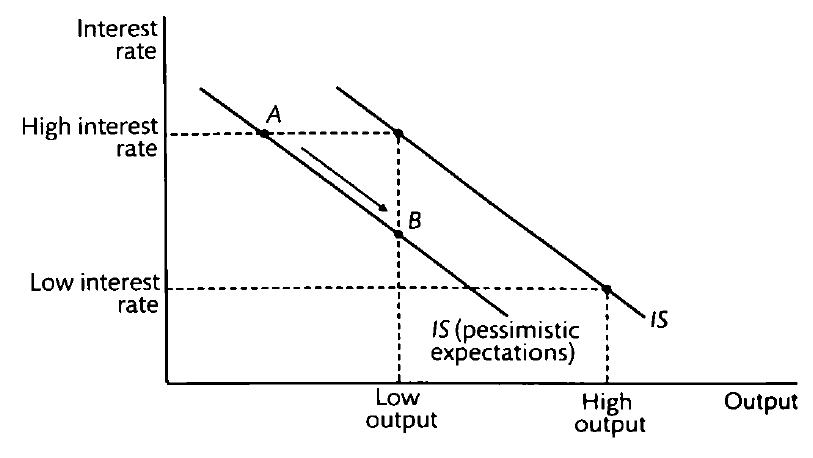
\includegraphics[width=0.7\textwidth]{./figures/aula6_fig1.PNG}
        \caption{Curva IS: efeitos de variações no otimismo e política econômica. Fonte: Carlin e Soskice (2014)}
    \end{figure}
\end{frame}

\begin{frame}
    {Demanda agregada: curva IS}
    \begin{itemize}
        \item Vimos como modelos de consumo e investimento se relacionam com características observadas empiricamente\bigskip
        \item E.g., maior volatilidade do investimento (comparado ao consumo) pode ser, parcialmente, explicada por fatores que influenciam decisões de gastos com investimento e pelo desejo dos consumidores de suavizar consumo, via poupança e empréstimos\bigskip
        \item Heterogeneidade de consumidores: alguns impacientes (com dificuldade de poupar), outros são prudentes (poupam por motivos precaucionários)\bigskip
        \item Governo contribui para suavização do consumo via provisão de benefício-desemprego\bigskip
        \item Restrições de crédito (para firmas e consumidores) ajudam a melhor alinhar modelos de consumo e investimento com evidências empíricas
    \end{itemize}
\end{frame}

\section{Oferta agregada: curva de Phillips}
\begin{frame}
    {Oferta agregada: curva de Phillips}
    \begin{itemize}
        \item Modelo WS-PS de fixação de preços e salários: utilizado para determinar nível de equilíbrio de produto agregado\bigskip
        \item A partir de WS-PS, derivamos a curva de Phillips - utilizada para modelar inflação de preços e de salários\bigskip
        \item Modelo mostra que salários, ao desemprego de equilíbrio, são maiores que salário de reserva\bigskip
        \item Portanto, há desemprego involuntário\bigskip
        \item Com competição monopolística no mercado de bens, firmas cobram um \emph{mark-up} sobre seus bens e, portanto, fazem lucros acima dos normais
    \end{itemize}
\end{frame}

\begin{frame}
    {Oferta agregada: curva de Phillips}
    \begin{itemize}
        \item Equilíbrio de médio prazo: taxa de desemprego é tal que fixadores de preços e salários estão satisfeitos com salário real vigente\bigskip
        \item Salário real é constante - salários e preços crescem à mesma taxa: inflação constante\bigskip
        \item Inflação poderia ser constante e zero e, neste caso, preços e salários permaneceriam inalterados\bigskip
        \item No entanto, economias são tipicamente caracterizadas por inflações positivas
    \end{itemize}
\end{frame}

\begin{frame}
    {Oferta agregada: curva de Phillips}
    \begin{itemize}
        \item \hlight{Relação de fixação de salários (WS)}:
        \begin{equation}
            W = P^e F(u,z)
        \end{equation}
        \item Fatores que pressionam salários incluem variáveis institucionais, de política, estruturais e choques\bigskip
        \item Curva WS desloca-se p/ baixo, reduzindo desemprego de equilíbrio, quando:\medskip
        \begin{enumerate}
            \item Queda no nível de benefícios desemprego ou em sua duração\medskip
            \item Queda na desutilidade do esforço: melhorias nas condições de trabalho aumentam o custo da perda de trabalho\medskip
            \item Menores proteções legais a sindicatos (reduzindo seus \emph{mark-ups})\medskip
            \item Sindicatos mais fracos: menor densidade de sindicatos ou menor cobertura de barganhas coletivas
        \end{enumerate}
    \end{itemize}
\end{frame}

\begin{frame}
    {Oferta agregada: curva de Phillips}
    \begin{itemize}
        \item \hlight{Relação de fixação de preços (PS)}:
        \begin{equation}
            P = (1 + \mu)\frac{W}{\lambda}
        \end{equation}
        \item Assumimos que \emph{mark-up} e produtividade do trabalho, $\lambda$, constantes - se $Y = N$, então, $\lambda = 1$\bigskip
        \item Curva PS horizontal\bigskip
        \item Curva PS desloca-se para cima, reduzindo desemprego de equilíbrio, quando:\medskip
        \begin{enumerate}
            \item Queda no \emph{mark-up}, $\mu$\medskip
            \item Aumento na produtividade do trabalho, $\lambda$
        \end{enumerate}
    \end{itemize}
\end{frame}

\begin{frame}
    {Oferta agregada: curva de Phillips}
    \begin{figure}
        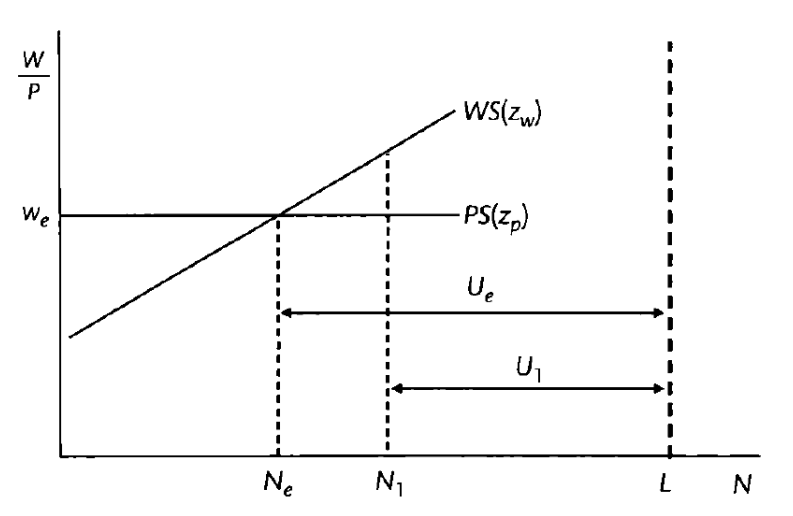
\includegraphics[width=0.7\textwidth]{./figures/aula14_fig1.PNG}
        \caption{Emprego e desemprego de equilíbrio. Fonte: Carlin e Soskice (2014)}
    \end{figure}
\end{frame}

\begin{frame}
    {Oferta agregada: curva de Phillips}
    \begin{itemize}
        \item Flutuações na demanda agregada podem causar desvios do equilíbrio de médio prazo - \hlight{ciclos econômicos induzidos por demanda}\bigskip
        \item Preços e salários não se ajustam automaticamente para manter o desemprego de equilíbrio: existência de rigidezes nominais\bigskip
        \item Salários são fixados periodicamente e empregadores não cortam salários nominais quando desemprego aumenta\bigskip
        \item Preços: flutuações de DA levam a ciclos se firmas respondem a variações de demanda alterando produto e emprego\bigskip
        \item Se preços e salários se alteram mas o produto não muda não observaríamos ciclos induzidos por demanda (caso clássico)
    \end{itemize}
\end{frame}

\begin{frame}
    {Oferta agregada: curva de Phillips}
    \begin{itemize}
        \item Possível explicação para ciclos induzidos por demanda: firmas, sob competição imperfeita, acham lucrativo responder a deslocamentos de demanda alterando produção\bigskip
        \item Rigidez de preços: relutância das firmas em alterar preços diante de variações de DA\bigskip
        \item Curva de demanda que uma firma em mercado imperfeito se depara é deslocada por choques à DA, do tipo que discutimos na curva IS\bigskip
        \item Em geral, deslocamento da curva de demanda de uma firma irá alterar preço e quantidade que maximizam seus lucros\bigskip
        \item Como preço desta firma excede seu custo marginal, a firma pode optar por não alterar seus preços - decisão depende de um \emph{trade-off} entre custos e benefícios de alterar preços
    \end{itemize}
\end{frame}

\begin{frame}
    {Oferta agregada: curva de Phillips}
    \begin{itemize}
        \item Existência de custos associados à alteração de preços: e.g., \hlight{custos de menu}\bigskip
        \item Mesmo que tecnologia de ajuste de preços a baixo custo esteja disponível, firma pode se preocupar em perder consumidores para firmas concorrentes que produzem bens similares caso estas não o façam\bigskip
        \item Dado que os benefícios de alterar preços são, provavelmente, modestos sob competição imperfeita, os custos não precisam ser elevados para compensarem os benefícios\bigskip
        \begin{enumerate}
            \item Taylor (1999): firmas americanas ajustam preços apenas anualmente e de forma dessincronizada (preços escalonados)\medskip
            \item Dhyne et al. (2006): resultados similares para área do Euro\medskip
            \item Moura e Rossi Jr. (2010): resultados similares para Brasil\medskip
            \item Estudos apontam heterogeneidade entre setores na duração de preços (serviços - maior grau de rigidez; alimentos não-processados e energia - menor grau de rigidez)
        \end{enumerate} 
    \end{itemize}
\end{frame}

\begin{frame}
    {Oferta agregada: curva de Phillips}
    \begin{itemize}
        \item Do modelo WS-PS derivamos a curva de Phillips (PC):
        \begin{equation}
            \pi_t = \pi_t^e - \alpha(u_t - u_n)
        \end{equation}
        \item PC relaciona desvio da taxa de inflação observada da expectativa inflacionária com desvios do desemprego com relação à taxa natural\bigskip
        \item Assumimos que produtividade do trabalho é constante $\Rightarrow$ variações no produto são refletidas em variações um-para-um no emprego\bigskip
        \item No entanto, não existe uma relação um para um entre variações de produto agregado e emprego\bigskip
        \item \hlight{Lei de Okun}: relação empírica entre variações na DA, produto e taxa de desemprego
    \end{itemize}
\end{frame}

\begin{frame}
    {Oferta agregada: curva de Phillips}
    \begin{itemize}
        \item Dada lei de Okun, podemos reescrever PC em termos de produto, em vez de desemprego\bigskip
        \item Temos a seguinte relação:
        \[
            u \equiv 1 - \frac{N}{L} \Rightarrow N = L(1 - u)
        \]
        \item Pela função de produção, obtemos:
        \[
            Y = N = L(1 - u)
        \]
        \item Quando taxa de desemprego é igual à natural, $u_n$, o emprego é dado por $N_n = L(1-u_n)$ e, portanto, o produto é $Y_n = L(1 - u_n)$        
    \end{itemize}
\end{frame}

\begin{frame}
    {Oferta agregada: curva de Phillips}
    \begin{itemize}
        \item Chamemos $N_n$ o nível natural de emprego e $Y_n$ o nível natural de produto, ou \hlight{produto natural} ou \hlight{produto potencial}\bigskip
        \item Podemos, então, obter uma relação em termos do desvio do produto com relação ao seu nível natural (\hlight{hiato do produto}):
        \begin{equation}
            Y - Y_n = L[(1 - u) - (1 - u_n)] = -L(u - u_n)
        \end{equation}
        \begin{enumerate}
            \item Desemprego em seu nível natural: produto igual ao natural (hiato do produto é zero)\medskip
            \item Desemprego acima da taxa natural: produto abaixo do potencial (hiato negativo)\medskip
            \item Desemprego abaixo da taxa natural: produto acima do potencial (hiato do produto positivo)
        \end{enumerate}
    \end{itemize}
\end{frame}

\begin{frame}
    {Oferta agregada: curva de Phillips}
    \begin{itemize}
        \item Podemos reescrever a relação anterior da seguinte forma:
        \[
          N_t - N_{t-1} = L(1 - u_t) - L(1 - u_{t-1}) = -L(u_t - u_{t-1})  
        \]
        \item Portanto:
        \[
            \frac{N_t - N_{t-1}}{N_{t-1}} = -\frac{L}{N_{t-1}}(u_t - u_{t-1})
        \]
        \item Lado esquerdo: taxa de crescimento do nível de emprego $g_N$\bigskip
        \item Pela função de produção adotada: $g_Y = g_N$\bigskip
        \item Note que $L/N_{t-1}$ é um número próximo da unidade
    \end{itemize}
\end{frame}

\begin{frame}
    {Oferta agregada: curva de Phillips}
    \begin{itemize}
        \item Portanto:
        \begin{align*}
          g_Y &\approx -(u_t - u_{t-1}), \\
          u_t - u_{t-1} &\approx - g_Y
        \end{align*}
        \item Relação entre produto e desemprego conhecida como \hlight{lei de Okun}\bigskip
        \item Como é corroborada empiricamente?
    \end{itemize}
\end{frame}

\begin{frame}
    {Oferta agregada: curva de Phillips}
    \begin{figure}
        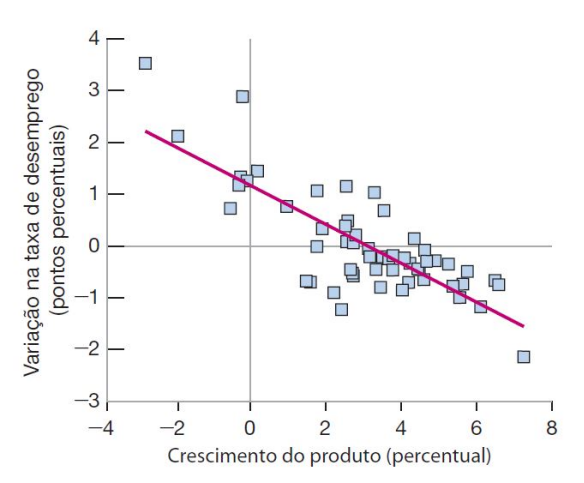
\includegraphics[width=0.5\textwidth]{./figures/aula14_fig2.PNG}
        \caption{Variações na taxa de desemprego $\times$ crescimento do PIB, EUA (1960-2014). Fonte: Blanchard (2017)}
    \end{figure}
\end{frame}

\begin{frame}
    {Oferta agregada: curva de Phillips}
    \begin{itemize}
        \item Linha de regressão para economia norte-americana (1960-2014):
        \[
            u_t - u_{t-1} = -0,4(g_Y - 3\%)
        \]
        \item Relação negativa entre variação do desemprego e crescimento do produto, mas com elementos adicionais:\medskip
        \begin{enumerate}
            \item Crescimento anual do PIB deve ser de pelo menos 3\% para evitar que taxa de desemprego se eleve. Isso deve-se a dois fatores que ignoramos até então: crescimento da força de trabalho e crescimento da produtividade do trabalho. Para manter taxa de desemprego constante, o crescimento do PIB deve ser igual à soma do crescimento da força de trabalho com o da produtividade do trabalho\medskip
            \item Coeficiente angular é -0,4 (e não -1). Ou seja, crescimento do PIB 1\% acima do normal leva a uma redução na taxa de desemprego de apenas 0,4\%, em vez de uma redução de 1\%
        \end{enumerate}
    \end{itemize}
\end{frame}

\begin{frame}
    {Oferta agregada: curva de Phillips}
    \begin{itemize}
        \item Portanto, curva de Phillips pode ser reescrita da seguinte forma:
        \begin{equation}
            \pi_t - \pi_t^e = \frac{\alpha}{L_t}(Y_t - Y_n)
        \end{equation}
        \item Sob a hipótese de expectativas adaptativas:
        \begin{equation}
            \pi_t - \pi_{t-1} = \frac{\alpha}{L_t}(Y_t - Y_n)
        \end{equation}
    \end{itemize}
\end{frame}

\begin{frame}
    {Oferta agregada: curva de Phillips}
    \begin{itemize}
        \item Choque positivo de DA: elevação do desemprego acima do nível de equilíbrio e, portanto, taxa de inflação aumenta\bigskip
        \item Protocolo temporal de eventos:
        \begin{align*}
            \varepsilon_t^d &\Rightarrow \Delta Y, \Delta N \\
            \text{Próxima rodada salarial} &\Rightarrow \Delta W \\
            \text{Imediatamente após rodada salarial} &\Rightarrow \Delta P
        \end{align*}
        \item Curva de Phillips modela, precisamente, este comportamento
    \end{itemize}
\end{frame}

\begin{frame}
    {Oferta agregada: curva de Phillips}
    \begin{figure}
        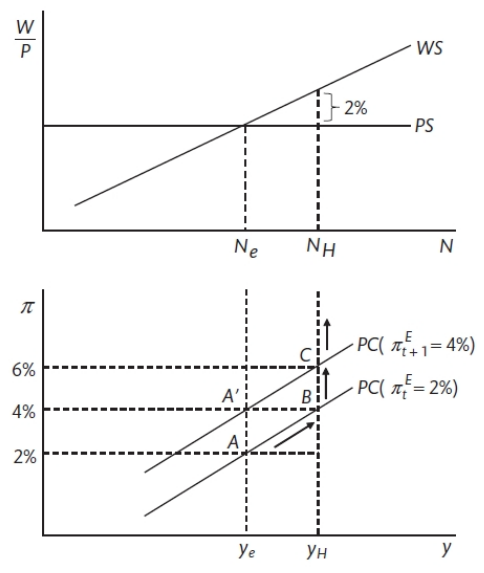
\includegraphics[width=0.37\textwidth]{./figures/aula14_fig3.PNG}
        \caption{Derivação da curva de Phillips. Fonte: Carlin e Soskice (2014)}
    \end{figure}
\end{frame}

\begin{frame}
    {Oferta agregada: curva de Phillips}
    \begin{itemize}
        \item Cada curva de Phillips mostra um conjunto factível de produto agregado e inflação para uma dada taxa de inflação esperada (expectativas adaptativas: defasada)\bigskip
        \item Cada curva de Phillips de expectativas adaptativas é definida por duas características:\medskip
        \begin{enumerate}
            \item Taxa de inflação defasada ($\pi_{t-1}$)\medskip
            \item Inclinação da curva WS, que fixa a inclinação da PC. Curva de Phillips é mais inclinada quando curva WS é mais inclinada
        \end{enumerate}
    \end{itemize}
\end{frame}

\begin{frame}
    {Oferta agregada: curva de Phillips}
    \begin{itemize}
        \item Curva de Phillips:
        \begin{align*}
            \pi_t &= \pi_t^e + \kappa(y_t - y_n) \\
            \pi_t &= \pi_{t-1} + \kappa(y_t - y_n) \tag{Expectativas adaptativas}
        \end{align*}
        \item Curva de Phillips desloca-se para cima ou para baixo quando inflação defasada é alterada\bigskip
        \item Inclinação depende de $\kappa \equiv \alpha/L$ que, por sua vez, reflete a inclinação da curva WS
    \end{itemize}
\end{frame}

\begin{frame}
    {Oferta agregada: curva de Phillips}
    \begin{itemize}
        \item Evidência empírica de dinâmica inflacionária: variações no produto (e emprego) são seguidas por variações na inflação: produto precede inflação e inflação é persistente\bigskip
        \item Consistente com a evidência, PC mostra que inflação corrente depende da inflação defasada, $\pi_{t-1}$, e do hiato do produto, $\tilde{y}_t$, (que reflete a diferença entre desemprego observado e taxa natural de equilíbrio)
    \end{itemize}
\end{frame}

\section{Aplicações}
\begin{frame}
    {Choques na ausência de uma autoridade monetária}
    \begin{itemize}
        \item Veremos que um BC sob metas de inflação (IT - \emph{inflation targeting}) irá diagnosticar a natureza de um choque e responderá ajustando a taxa básica de juros (instrumento de política monetária)\bigskip
        \item Para motivar a introdução de uma autoridade monetária que objetiva estabilizar a economia, vejamos o que acontece quando o sistema econômico é perturbado por um choque de oferta ou de demanda em sua ausência\bigskip
        \item Choque de DA: deslocamento da curva ou ao longo da curva IS\bigskip
        \item Choque de OA: deslocamentos da curva PS ou WS
    \end{itemize}
\end{frame}

\begin{frame}
    {Choques de demanda agregada}
    \begin{itemize}
        \item Choque positivo de DA: deslocamento da IS para direita\bigskip
        \item A hipótese de ausência de uma autoridade monetária reflete-se no fato de que curva IS permanece na nova posição após o choque e, portanto, taxa de juros real é mantida constante em seu nível inicial ($r_e$)\bigskip
        \item Assuma economia em um nível inicial de produto potencial de $y_e$ e inflação defasada de 2\% \bigskip
        \item IS desloca-se para nova posição IS'
    \end{itemize}
\end{frame}

\begin{frame}
    {Choques de demanda agregada}
    \begin{figure}
        \href{https://bookdown.org/robohay/economicsnotes/Figures/Supply/demandshock.jpg}{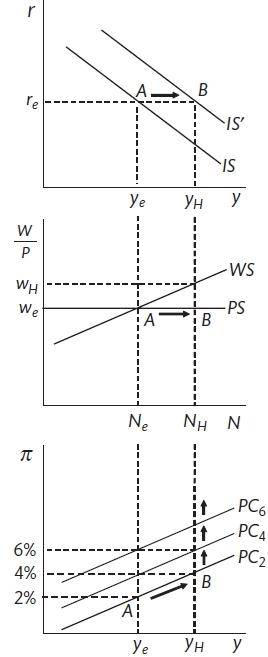
\includegraphics[width=0.18\textwidth]{./figures/aula14_fig4.jpg}}
        \caption{\href{https://bookdown.org/robohay/economicsnotes/Figures/Supply/demandshock.jpg}{Choque positivo de demanda agregada}. Fonte: Carlin e Soskice (2014)}
    \end{figure}
\end{frame}

\begin{frame}
    {Choques de demanda agregada}
    \begin{itemize}
        \item Choque de DA é acompanhado por uma espiral inflacionária\bigskip
        \item Com PIB acima do nível potencial (em $y_H$), o mercado de trabalho está em desequilíbrio (hiato entre curvas WS e PS em todos os períodos)\bigskip
        \item Salários e preços são ajustados primeiro quando fixadores de salários tentam alcançar um salário real mais elevado ($w_H$) e, segundo, à medida que firmas pressionam por aumento de preços para restaurar margens de lucro (o que implica que salário real seja mantido em $w_e$)\bigskip
        \item Com juro real constante em $r_e$, um choque positivo de DA é associado a emprego mais elevado e espiral inflacionária\bigskip
        \item Sem intervenção de um BC, não há nada que previna uma espiral inflacionária (ou deflacionária) de acontecer
    \end{itemize}
\end{frame}

\begin{frame}
    {Choques de oferta agregada}
    \begin{itemize}
        \item Choque de OA pode ser modelado como um deslocamento:\medskip
        \begin{enumerate}
            \item Função de produção: choque tecnológico ou de produtividade ($\Delta \lambda$)\medskip
            \item Curva de fixação de salários: deslocamento no poder de barganha de trabalhadores para empregadores ou em qualquer outro fator que pressione salários ($z$)\medskip
            \item Curva de fixação de preços: competição mais intensa no mercado de bens (e.g. $\downarrow \mu$) ou variação em qualquer outro fator que pressione preços\bigskip
        \end{enumerate}
        \item Exemplo: reformas no mercado de trabalho no UK na década de 1980\bigskip
        \item Reformas incluíram redução do poder de sindicatos, maior dificuldade de acesso ao seguro desemprego e redução no nível do benefício\bigskip
        \item Reformas que têm efeito de deslocar curva de fixação de salários para a direita, reduzindo o nível de desemprego de equilíbrio
    \end{itemize}
\end{frame}

\begin{frame}
    {Choques de oferta agregada}
    \begin{figure}
        \href{https://data.oecd.org/chart/6Ujt}{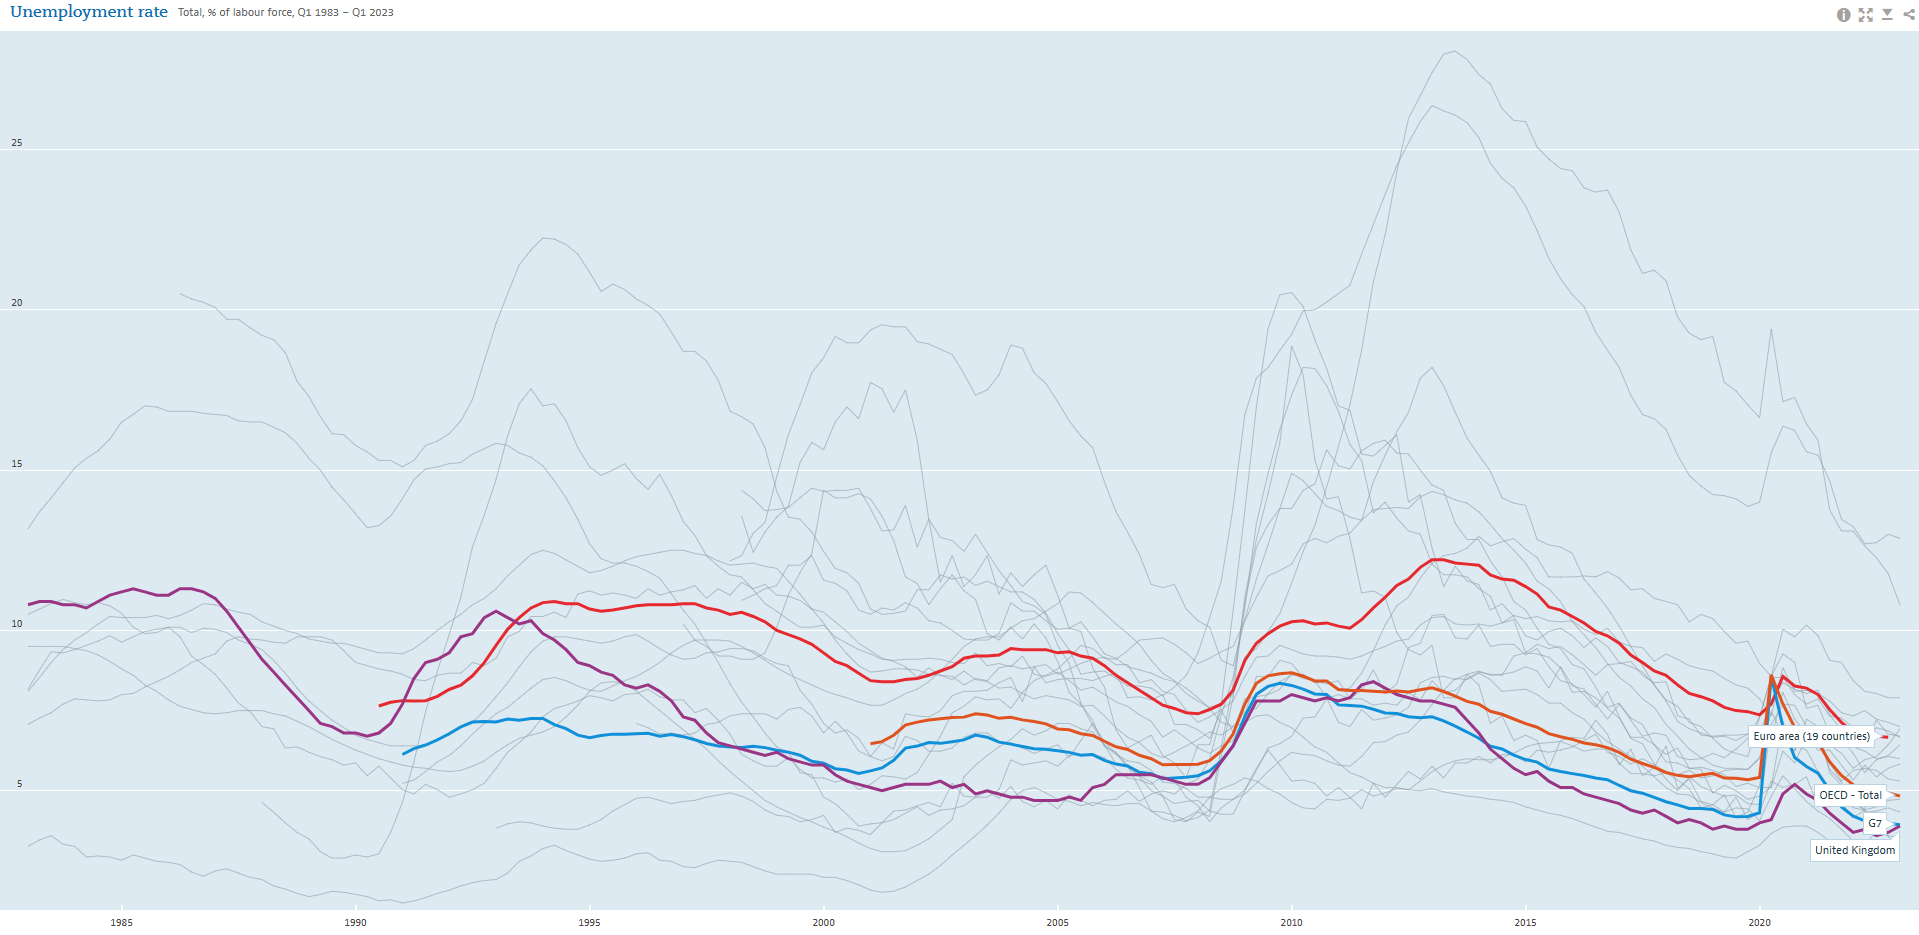
\includegraphics[width=0.9\textwidth]{./figures/aula14_fig5.PNG}}
        \caption{\href{https://data.oecd.org/chart/6Ujt}{Taxa de desemprego (1983-2023)}. Fonte: OCDE}
    \end{figure}
\end{frame}

\begin{frame}
    {Choques de oferta agregada}
    \begin{itemize}
        \item Situação inicial: equilíbrio natural $y_e$ e inflação defasada de 2\%\bigskip
        \item Choque positivo de OA que desloca curva WS para baixo\bigskip
        \item Isso, por sua vez, aumenta nível de equilíbrio de médio prazo do emprego e produto agregados\bigskip
        \item Na ausência de uma autoridade monetária, taxa real de juros é mantida constante em $r_e$ após o choque\bigskip
        \item Ao nível original de produto natural, $y_e$, há um hiato negativo entre curvas WS e PS\bigskip
        \item Fixadores de salários responderão ao hiato reduzindo demandas por salários reais, $w_L$\bigskip
        \item O fazem pois agora há uma maior competição por postos de trabalho e um custo maior associado à perda de emprego
    \end{itemize}
\end{frame}

\begin{frame}
    \begin{itemize}
        \item Salários nominais não aumentam e, de forma a manter margem de lucro constantes, firmas não alteram preços\bigskip
        \item Portanto, inflação cai de 2\% para 0\% e PC desloca-se para baixo\bigskip
        \item Nos períodos subsequentes, o ajuste é similar a um choque adverso de DA\bigskip
        \item Inflação será reduzida em cada período\bigskip
        \item Este processo será mantido indefinidamente, enquanto o PIB é mantido abaixo do novo valor de equilíbrio de médio prazo, i.e., o desemprego não pode ser mantido permanentemente acima do nível natural sem causar uma espiral deflacionária
    \end{itemize}
\end{frame}

\begin{frame}
    {Choques de oferta agregada}
    \begin{figure}
        \href{https://bookdown.org/robohay/economicsnotes/Figures/Supply/supplyshock.jpg}{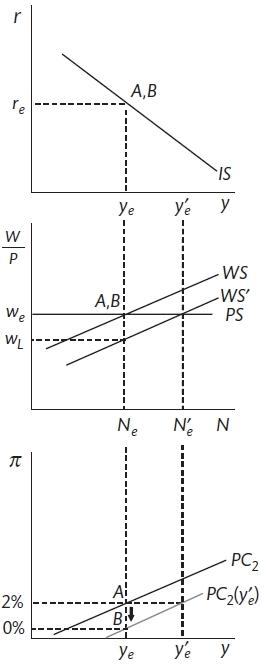
\includegraphics[width=0.18\textwidth]{./figures/aula14_fig6.jpg}}
        \caption{\href{https://bookdown.org/robohay/economicsnotes/Figures/Supply/supplyshock.jpg}{Choque positivo de oferta agregada}. Fonte: Carlin e Soskice (2014)}
    \end{figure}
\end{frame}

\begin{frame}
    {Choques de oferta agregada}
    \begin{itemize}
        \item Choque positivo de OA é caracterizado por aumento no PIB potencial e no emprego de equilíbrio de médio prazo\bigskip
        \item Vimos que um choque positivo de OA é associado a uma desaceleração inflacionária ao \hlight{nível inicial de produto agregado} $y_e$\bigskip
        \item Se o choque de OA é permanente, então, a economia é capaz de operar com um desemprego mais baixo e inflação constante
    \end{itemize}
\end{frame}

\section{Bibliografia}
\begin{frame}{\emoji{books} Bibliografia}
    \begin{itemize}                
        \item BLANCHARD, O. Macroeconomia. 7.ed. São Paulo: Pearson Education do Brasil, 2017\medskip                
        \item CARLIN, W.; SOSKICE, D. Macroeconomics: Institutions, instability, and the financial system. Oxford, UK: Oxford University Press, 2015\medskip        
        \item DHYNE, E.; ÀLVAREZ, H.; VERONESE, D.; HOFFMANN, J.; JONKER, N.; LUNNEMANN, P.; RUMLER, F.; VILMUNEN, J. Price changes in the Euro Area and the United States: some facts from Individual Consumer Price data. Journal of Economic Perspectives 20(2), 171-192, 2006\medskip
        \item MOURA, M.; ROSSI JR., J. Price-setting policy determinants: micro-evidence from Brazil. Economia Aplicada 14, 169-182, 2010\medskip
        \item TAYLOR, J.B. Staggered price and wage setting in Macroeconomics. in J.B. Taylor, M. Woodford, eds., Handbook of Macroeconomics 1341-1397, Elsevier, New York (1999)         
    \end{itemize}
\end{frame}
\end{document}